% !TEX root = master.tex
Ever since the 1920 Great Debate on the nature of nebulae, it has been known that the Milky Way is not the entirety of our universe, that there are indeed other `island universes' called galaxies \citep{berendzen_man_1976}. 

Modern ideas on how these immense structures formed describe quantum fluctuations in the very early universe becoming stretched during the inflationary period \citep{liddle_introduction_2003}. Significant gravitational perturbations arise out of these expanded wrinkles in space and after some time enough matter is accumulated and star formation can begin \citep{coles_cosmology:_2002}.

It is therefore important to understand the nature of galaxy formation if we wish to test cosmological models, since there is a direct relationship between large scale structure formation and cosmological parameters.

The most popular cosmology currently in use, $\Lambda$CDM (Cold Dark Matter), correctly predicts the existence of the CMB, the distribution of galaxies and the abundances of light elements \citep{liddle_introduction_2003} >>better reference<<. However, $\Lambda$CDM simulations diverge from observation at the galactic scale, predicting excessive numbers of dwarf galaxies \citep{silk_massive-black-hole-velocity-dispersion_2010} and too few massive bulgeless galaxies with thin disks \citep{kormendy_bulgeless_2010}.

Constraining galaxy properties with observation allows one to constrain or perhaps modify aspects of the $\lambda$CDM and hence lead to a more certain understanding of the early universe. >>More specifics<<

\subsection{Galaxy Properties}
Galaxies are not all indistinct clumps of stars but can take on a range of diverse structures \citep{hubble_no._1926}. Most galaxies can be crudely classified into three broad categories based on stellar content and morphology: Elliptical, Spiral and Irregular. 

Ellipticals are centrally condensed objects with a typical diameter from under 1 kpc to 200 kpc \citep{carroll_introduction_2007} and a smooth almost featureless luminosity profile. Ellipticals, as their name suggests, exhibit an elliptical shape range from ellipticity $\epsilon = 1$ (spheroidal E0) to around $\epsilon = 0.7$ (very oblate E7). 
Ellipticals contain little gas and hence little ongoing star formation due to their low gravitational binding energy \citep{crocker_molecular_2011}. 
Because they contain mostly old stars, ellipticals have higher metallicity and have moved off onto the red sequence, hence they are commonly called `red and dead' \citep{binney_galactic_1998}.  

\begin{figure}
	\label{galaxy type pictures}
\end{figure}

Spirals, in contrast, are very different to ellipticals in their structure. They are blueish disk galaxies usually with a redder central bulge and spiral arms with vivid dust lanes \citep{sparke_galaxies_2000}. The spiral arms are in fact density perturbations travelling around the disk, where the the increase in gas density initiates local star formation \citep{kennicutt_star_1998}. They therefore contain many more younger  main sequence stars, typically giving spirals a bluer hue of $0.4\lesssim B-V \lesssim 0.8$, where $B$ and $V$ are the magnitudes in the `blue' and `visible' wavebands in the UBV photometric system \citep{sparke_galaxies_2000}.

\subsection{S0s and Classification}
The traditional method of classifying galaxies is the Hubble Tuning Fork \citep{hubble_no._1926}. Hubble arranged galaxies from `early' to `late' types with the implicit assumption that all galaxies evolved that way in time. We now know that this transformation from early to late type is impossible since there is no way for ellipticals to increase their negligible angular velocity to match that of fast rotating spirals \citep{carroll_introduction_2007}. 

Spirals are sorted by the bulge size and tightness of their spiral arms and ellipticals by their ellipticity. On this continuous fork, an intermediate `lenticular' class is necessarily created. 
\begin{figure}
	\label{hubble_fork}
\end{figure}
Lenticulars, or S0 galaxies, are observed to share the stellar content of ellipticals but the structure and kinematics of spirals. They are disk galaxies but have a smooth brightness profile free from spiral arms \citep{blanton_physical_2009}. S0s can be dusty and have few HII regions associated with young stars \citep{degraaff_galaxy_2007}. Together with a high metallicity, these properties give the galaxy a `red and dead' appearance with $0.7\lesssim B-V \lesssim 0.9$.

Due to their similarity with ellipticals, there have been many misclassifications of S0s with low inclinations (side-on) \citep{laurikainen_multicomponent_2005}. 
S0s do not have significant emission on the H$\alpha$ line and estimates of dynamical mass become challenging \citep{dressler_rotational_1983}. S0s have a central spheroidal component or bulge, which on average, is flatter than an elliptical and usually brighter than its disk unlike spiral bulges \citep{dressler_galaxy_1980}.

\subsection{Photometry}
Morphological classification remains, by its qualitative nature, subjective and open to interpretation \citep{naim_automated_1995}. Using the quantitative measure of galaxy luminosity profiling minimises disagreement between observers and helps to quantify physical properties with more certainty. 

Profiles are generated by isophotal analysis, whereby one fits thin ellipses of equal intensity (an `isophote') to the image, working outwards from the previously established centroid. Plotting the average isophote intensity against geometric mean radius to generate a 1D intensity profile \citep{peng_detailed_2002}. Now galaxy can be fitted by mathematical models and the resulting parameters analysed. 

De Vaucouleurs was one of the first to propose his $R^{1/4}$ model for galaxy light distribution \citep{de_vaucouleurs_revised_1963}. This model was successful in fitting elliptical galaxies and is still used today with bulges of S0 and spiral galaxies \citep{allen_millennium_2006}. However, this model does not describe all bulges well and an exponential model best describes disks! Given this variation in model parameters, the De Vaucouleurs model can be generalised to a \sersic $R^1/n$ model \citep{sersic_atlas_1968}.
\begin{equation}
		I(R) = I_{e} \rm{exp}\left\{-b_{n}\left[\left(\frac{R}{R_{e}}\right)^{1/n} - 1\right]\right\},
\end{equation}
where $I(R)$ is the intensity at radius $R$, $n$ is the Sersic index, $R_e$ is the effective radius which encloses half the total intensity, $I_e$ is the intensity at $R_e$ and $b_n$ is defined such that $\Gamma(2n) = 2\gamma(2n, b_n)$, where $\Gamma$ is the complete gamma function and $\gamma$ is the incomplete gamma function.
\begin{figure}[!ht]
		\centering
		% 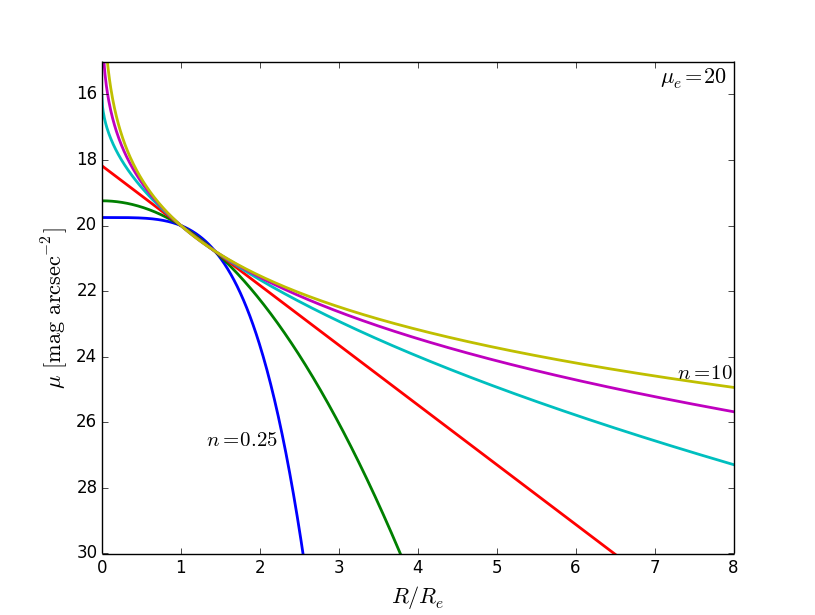
\includegraphics[width=\linewidth]{sersic_mags}
		\caption{Magnitude profiles of Sersic indices from 0.25 to 10}
		\label{fig:sersic_mags}
	\end{figure}
\ref{fig:sersic_mags} shows the effects of adjusting the \sersic index with respect to a constant effective surface brightness. As $n$ becomes smaller, the light becomes less centrally concentrated and lower in central intensity \citep{graham_concise_2005}. 

Most galaxies do not consist purely of one component \citep{laurikainen_multicomponent_2005}, but include several, such as disks, bulges and bars. The \sersic model has been found to fit all of these components with low residuals and is reliably used to classify galaxies into morphological type \citep{peng_detailed_2010}.

\subsection{The origins of S0 Galaxies}
The origin of lenticular galaxies remains a highly active area of research. Logic dictates two possibilities for S0 formation: Either they formed in the same manner as ellipticals at the start of the galaxy formation era or they have since evolved from spirals by some unknown mechanism \citep{burstein_k-band_2005}.

If S0s did indeed transform from spiral-like galaxies, then a corresponding increase in the population of spirals should be seen over increasing redshift. This trend has been observed, showing an increase in early-types with look-back time \citep{dressler_evolution_1997}.

There is also evidence from Tully-Fisher Relation (TFR), in which galaxy luminosity is related to maximum rotational velocity \citep{tully_new_1977}. This relation is tightly defined for local spirals, with a small intrinsic scatter, as $0.43 \pm 0.03$ mag averaged over SDSS griz bands \citep{pizagno_tully-fisher_2007}. Now that reliable TFRs have been constructed or S0s \citep{bedregal_tullyfisher_2006}, the existence of an offset from spirals is confirmed. S0s are fainter than spirals by an average of $0.85 \pm 0.19$ mag in the $i$-band, with a similar offset is found in the $g$ and $K_s$ bands \citep{rawle_s0_2013}. This offset can be interpreted as the cessation of star formation and subsequent fading of the disk.

Various mechanisms for quenching star formation have been proposed. Ram-pressure stripping removes the disk gas necessary for subsequent star formation \citep{gunn_infall_1972}; strangulation would remove larger reservoir of halo gas, having a slower and gentler impact on star formation; or the harsher minor merger of two spirals, exhausting a large amount of the interstellar medium (ISM)  \citep{bekki_unequal-mass_1998} to name but a few.

Given that the typical surface brightness of S0s has actually found to be greater than that of spirals \citep{burstein_k-band_2005}, this suggests that the bulge luminosity of S0s is too large to evolve from disk fading alone \citep{cortesi_planetary_2013}. The increased brightness favours minor mergers or galaxy harassment, where frequent high speed encounters strip disk gas and dump some of it at the centre \citep{moore_galaxy_1996}.

The well-known morphology-density relation \citep{dressler_galaxy_1980}, describes an increase in early types with projected surface density. This is to be expected if S0s result from galaxy interactions but S0s are observed in the field, suggesting that this may not be the whole story. If this is indeed the case, then either cluster based mechanisms such as ram-pressure stripping cannot be responsible for S0 formation, or there are multiple evolutionary paths to S0s operating in different environments. 

If the evolutionary mechanism is dependent on density, then there might be structural differences in S0 galaxies as a function of environment which can be used to probe evolutionary history.
>>>see head for good description of fading process<<<

\subsection{Truncation}
-infinite exp. doesn't describe completely, most disks
-three classes of truncation
-graphs of own truncated gals
-erwin



One feature, suitably sensitive to external interactions, is the outer structure of the disk \citep{pohlen_stellar_2004}. The outermost radii should be vulnerable to the effects of galaxy-galaxy interactions, late-time accretion and gas stripping, hence retaining an imprint of formation process. 

Disk galaxies have been known not to obey an infinitely extended exponential light distribution for 35 years \citep{van_der_kruit_optical_1979}. It has become apparent that most (79\% according to \citet{pohlen_cut-off_2001}) disk galaxies exhibit `truncations' or `breaks' in their otherwise smooth exponential profiles. 

S0 galaxy truncations can fall into three broad truncation classes: Type-I: single-exponential, Type-II: classicly truncated \citep{freeman_disks_1970} or Type-III: anti-truncated \citep{erwin_antitruncation_2005}. 
\begin{figure}
	\label{own sample examples on truncated types}
\end{figure}

Though early analysis indicated an even distribution of types in local S0s \citep{gutierrez_outer_2011}, when the cluster and field are analysed separately a distinct difference arises. While field S0s are divided roughly evenly between all three types, Virgo S0s appear to be completely devoid of type-IIs with $M_v < -17$ $f_{S0} = 0_{-0}^{+4}\%$ \citep{erwin_strong_2012}. Since type-IIIs are found to be equally common in both environments, the difference is made up of type-I profiles, making single-exponentials twice as common in the Virgo cluster than in the field. 

To account for such a drastic change in type population, either something in the (early) cluster transforms type-II into type-I or something prevents the opposite transition which is common in the field. Assuming cluster S0s originally had type-II truncated profiles, then a mechanism is required which erases said truncation. Harassment is a popular take ............

\subsection{Aims of Project}
- is it possible to find and classify truncations using a 1D profile method
-compare and contrast Virgo and Coma
-variation within the cluster
-search for a correlation between \sersic parameters and trunc. type

In this project, we investigate the feasibility of detecting and classifying truncations in the coma cluster S0s using a simple 1D bulge-disc decomposition procedure. 

\citet{erwin_strong_2012} used a sample of 24 S0s within the Virgo cluster. By studying Coma S0s we can select a larger number of S0s over a wide range of cluster-centric radii and hence compare and contrast the results with \citet{erwin_strong_2012}. 

In addition, we also investigate truncation type as a function of cluster-centric radius in an effort to see if the truncation mechanism also depends on cluster density as well as cluster membership.

Lastly, a search for a correlation between \sersic parameters and truncation type is investigated.

